\documentclass[10pt,a4paper]{article}
\usepackage[utf8]{inputenc}
\usepackage{amsmath}
\usepackage[document]{ragged2e}
\usepackage{amsfonts}
\usepackage{amssymb}
\usepackage{graphicx}
\usepackage[utf8]{inputenc}
\usepackage[english]{babel}
\usepackage{fancyhdr}

\author{PREM SAGAR S - AE14B021}
\title{Assignment 1 \\ Unconstrained Single Variable Optimization   Pipeline Problem}

\pagestyle{fancy}
\fancyhf{}
\fancyhead[LE,RO]{Assignment 1}
\fancyhead[RE,LO]{AE14B021}

\begin{document}
\maketitle
\justify

\section{Problem Description}
\begin{center}
 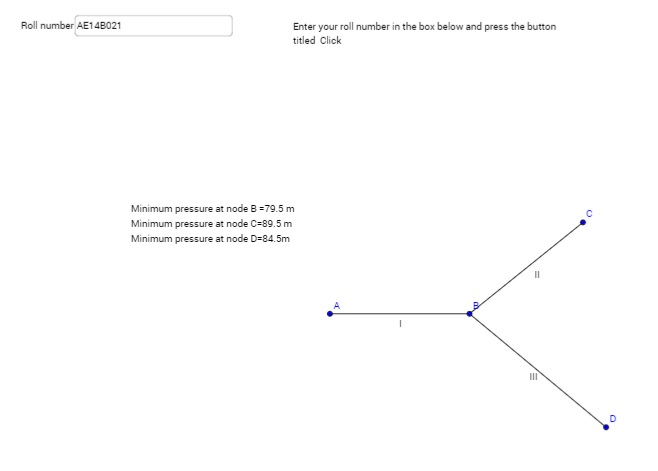
\includegraphics[scale=0.8]{p1}
\end{center}
 
\section{Heads at all nodes}
\begin{enumerate}
\item Node 1 :  
  \begin{equation}
   \begin{split}  
  H_1 = H_0 - \Delta H_{01} 
      = 100-\frac{4.457*10^8*300*9^{1.85}}{D_1^{4.87}} 
    \\  = 100-\frac{7.7895*10^{12}}{D_1^{4.87}}   
 \end{split} 
 \end{equation}

\item Node 2 :
\begin{equation} \begin{split}
 \newline  H_2 = H_1 - \Delta H_{12}    = H_1 - \frac{4.457*10^8*500*3^{1.85}}{D_2^{4.87}} \\ 
   =100-\frac{4.457*10^8*300*9^{1.85}}{D_1^{4.87}}- \frac{4.457*10^8*500*3^{1.85}}{D_2^{4.87}} \\ = 100-\frac{7.7895*10^{12}}{D_1^{4.87}}  -  \frac{ 1.7*10^{ 12}}{D_2^{4.87}} 
 \end{split} 
 \end{equation}
\item Node 3 : 
 \begin{equation}
   \begin{split}     H_3 = H_1 - \Delta H_{13}  = H_1 - \frac{4.457*10^8*400*2^{1.85}}{D_3^{4.87}} \\ =100-\frac{4.457*10^8*300*9^{1.85}}{D_1^{4.87}}-   \frac{4.457*10^8*400*2^{1.85}}{D_3^{4.87}} \\ =  100-\frac{7.7895*10^{12}}{D_1^{4.87}}- \frac{ 6.4269*10^{ 11}}{D_3^{4.87}} 
\end{split} 
 \end{equation}
\end{enumerate}

\section{ Cost function}

Given the cost function per unit length, we get the follwing expression for the total cost for the entire network.
\begin{equation}
 C = 1.2654 [300D_1^{1.327} +500D_2^{1.327}+400D_3^{1.327}] 
 \end{equation}
 
\section{ Formulation of the problem }

At the optimum, the heads must be the minimum specified in the problem. But, for the flow to sustain,  the constraint on $H_1$ is redundant because,
\newline  $H_1>H_2\geqslant 89.5m>79.5m$ and
 \newline  $H_1>H_3\geqslant 84.5m>79.5m$
 \newline Therefore, $H_2 = 89.5m$ and $H_3 = 84.5m$. The problem boils down to finding $H_1$.

 With these heads at nodes 2 and 3, the following relations for the diameters in terms of $H_1$ alone can be derived:
 \begin{equation}
   \begin{split} 
    D_1 = \frac{443.739}{{(100-H_1)}^\frac{1}{4.87}} \\   D_2 = \frac{324.664}{{(H_1-89.5)}^\frac{1}{4.87}}  \\   D_3= \frac{265.853}{{(H_1-84.5)}^\frac{1}{4.87}} 
   \end{split} 
 \end{equation}
The cost function can be written in terms of $H_1 $ alone, with all the constraints satisfied, the problem is now converted to an \textbf{ unconstrained optimization problem in one variable.} \newline
 \begin{equation}
   \begin{split} 
   C = 1.2654 [300( \frac{443.739}{{(100-H_1)}^\frac{1}{4.87}})^{1.327} +500(\frac{324.664}{{(H_1-89.5)}^\frac{1}{4.87}})^{1.327}  \\ +400( \frac{265.853}{{(H_1-84.5)}^\frac{1}{4.87}})^{1.327}]
%\\ =  [ \frac{1236196.2}{{(100-H_1)}^{0.272}} + \frac{816624.08}{{(H_1-89.5)}^{0.272}} +  \frac{626395.2}{{(H_1-84.5)}^{0.272}} ]
   \end{split} 
 \end{equation}
 Since $H_1<100m$ for the flow to sustain, our solution must have $100m>H_1>89.5m$. The optimal $H_1$  must be sought in this interval.
 
 \section{Optimal solution}
 
 \par The solution can be sought in multiple ways. Analytical method involves finding the point where the deriavative is zero. Numeraical methods include Uniform search method, Golden search method, Fibbinocci search method etc.
% \begin{itemize}
 %\item Since the interval to search is only about 10m, the cost function can be evaluated at multiple points by trial and error to search for the minimum. But this is inefficient and isn't quite a proper algorithm.
% \item \textbf{Golden Section Method:} The discussion here is posed in terms of searching for a minimum (searching for a maximum is similar) of a unimodal function. Unlike finding a zero, where two function evaluations with opposite sign are sufficient to bracket a root, when searching for a minimum, three values are necessary. The golden section search is an efficient way to reduce progressively the interval locating the minimum. The key is to observe that regardless of how many points have been evaluated, the minimum lies within the interval defined by the two points either side of the least value so far evaluated.
% \item \textbf{Fibbinocci Search method:} A very similar algorithm can also be used to find the extremum (minimum or maximum) of a sequence of values that has a single local minimum or local maximum. In order to approximate the probe positions of golden section search while probing only integer sequence indices, the variant of the algorithm for this case typically maintains a bracketing of the solution in which the length of the bracketed interval is a Fibonacci number. For this reason, the sequence variant of golden section search is often called Fibonacci search. \textbf{This could give faster convergence than the Golden search method with fewer iterations.}
% \end{itemize}
 
 \subsection{Solution by Uniform Search method}
\par The minimum of the cost function can be determined by choosing an interval of reasonable size, evaluating the cost at four equidistant points including the bounds. The equal part containing the highest cost can be eliminated. This is applicable only when the function is monotonous about the minimum. Once that part eliminated, the new band is divided again into three equal parts and the region containing the highest cost function is eliminated. This is done iteratively until we reach a convergent value for the cost function. The iterations for the problem with the initial band from 90m-99.5m is shown.
 \begin{center}
 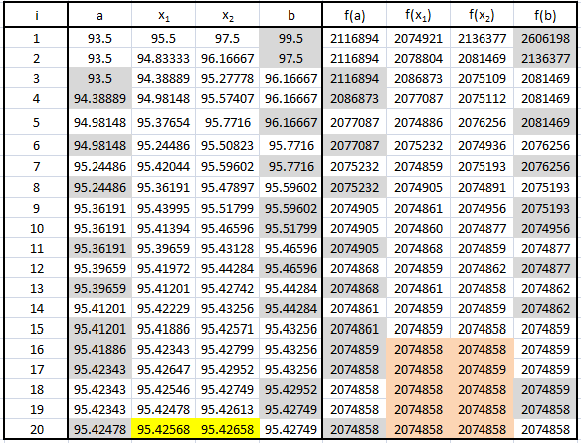
\includegraphics[scale=0.75]{m1}
  %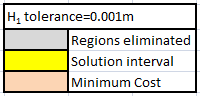
\includegraphics[scale=0.3]{m2}
\end{center}
\begin{center}
% 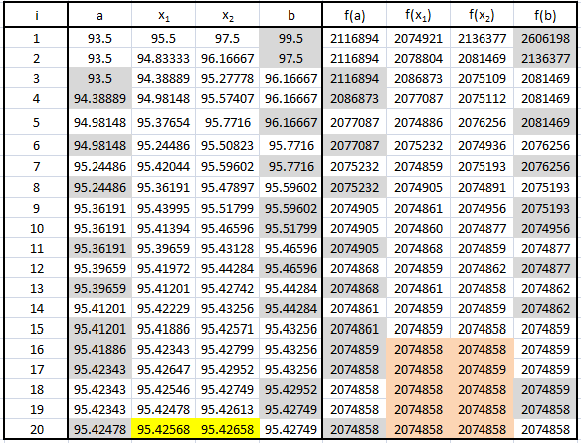
\includegraphics[scale=0.8]{m1}
  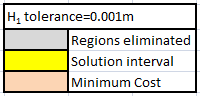
\includegraphics[scale=0.8]{m2}
\end{center}
 
 The cost function reaches convergence in the region 95.42568m to 94.42658m. We may as well take \textbf{95.43m} to be the optimum, since the residue was set to be 0.001m. So the optimum cost of the pipeline network is \textbf{INR 20,74,858.37}
 \newline The optimum diameters for the three links can be evaluated from equations (5) as below:
 
  \begin{center}
$D_1=324.80mm$  
 \newline  $D_2=225.27mm$  
 \newline   $D_3=162.69mm$  \newline
 \end{center}
  \subsection{Solution by Golden Search method}
  
  Divide interval into 3 sections by adding two internal points between ends. Evaluate the function at the two internal points x1 and x2. If f(x1)$ < $f(x2)
the maximum is between x1 and xmx. Redefine range xmn = x1, xmx = xmx. Set the following conditions:
(1) L = L1 + L2
(2) R = L/L2 = L2/L1.  Thus, R = (sqrt(5)-1)/2 = .61803. (Golden ratio). \textbf{This method reduces function evaluation because every successive iteration re-uses one of the previous internal values.}
 % \begin{center}
% 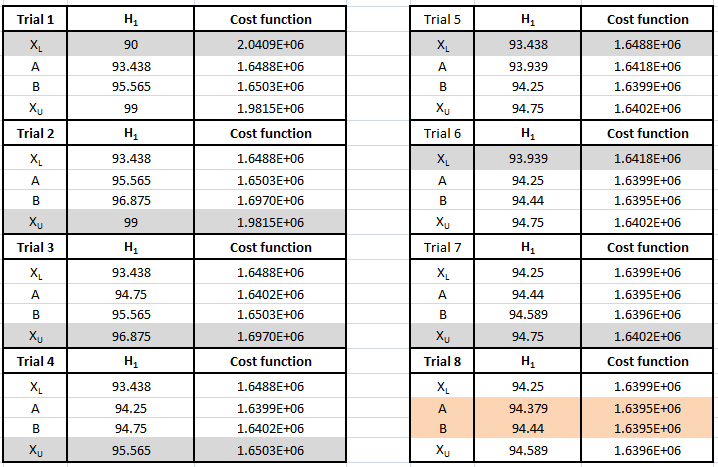
\includegraphics[scale=0.7]{golden}
%\end{center}

%\textbf{As can be seen, the solution reaches convergence faster than the previous method. }The cost function reaches convergence in the region 94.38m to 94.44m. We may as well take the average \textbf{94.41m} to be the optimum. There is not much of a huge difference from the previous method. So the optimum cost of the pipeline network is \textbf{INR 1.6395*10$^6$.}
% \newline The optimum diameters for the three links can be evaluated from equations (5) as below:
 
%\begin{center}
%$D_1=311.64mm$  
% \newline  $D_2=234.22mm$  
% \newline   $D_3=166.00mm$   \newline
 %\end{center}
 
  \subsection{Solution by Fibbinocci Search method}
  
 The Fibonacci search is based on the use of the Fibonacci number series. Each $n^{th}$  Fibonacci number is the sum of the preceding two numbers. The Fibonacci search begins by placing the experiments at a distance $d_1=\frac{F_{n-1}}{F_n}L$ from each end of the range of values, where L is the range of lengths. The interval with highest functional value is eliminated as done previously. The new interval is again split with  $d_2=\frac{F_{n-3}}{F_{n-1}}L$. This is done iteratively to reach convergence. 'n' can be chosen to obtain the solution interval in 'n-1' iterations. This method in the limiting case becomes the Golden search method. This reaches faster convergence because it removes bigger chunks of intervals compared to the previous methods and is thus, the optimal method.. 
% \begin{center}
 %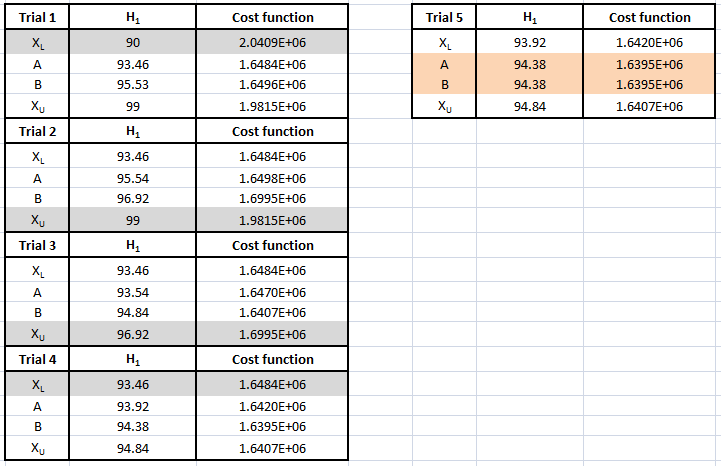
\includegraphics[scale=0.7]{fibbi}
%\end{center}

%This method reaches convergence interval much faster than the Golden search method making it the most \textbf{optimal method} to get the same optimal cost of \textbf{INR 1.6395*10$^6$.} The optimal solution can be taken as 94.38m. The diameters can  be calculated as below:

%\begin{center}
%$D_1=311.30mm$  
% \newline  $D_2=234.46mm$  
% \newline   $D_3=165.98mm$   \newline
% \end{center}
 
\end{document}
